\documentclass[14pt,a4paper]{extarticle}
%\documentclass[12pt,a4paper]{article}

\usepackage[utf8]{inputenc}
\usepackage[ukrainian]{babel}


\usepackage{amssymb}
\usepackage{physics}


\usepackage[active]{srcltx}
\usepackage[final]{pdfpages}

\usepackage[hidelinks]{hyperref}

\usepackage{verbatim}
%%%%%%%%%%%%%%%%%%%%%%%%%%%%%%%%%%%%%%%%%%%%%%%%%%%%%%%%%%%%%%%%%%
%\pagestyle{empty}                     %нумерацiя сторiнок i т.д.
\pagestyle{headings}                   %нумерацiя сторiнок вгорi зправа i т.д.
%\renewcommand{\baselinestretch}{1.5}   %мiжстрiчковий інтервал
%\parindent=7.5mm                      %абзацний відступ
 \righthyphenmin=2                     %перенос 2 останніх букв
 \pagenumbering{arabic}
 \tolerance=400
 \mathsurround=2pt
 \hfuzz=1.5pt
%%%%%%%%%%%%%%%%%%%%%%%%%%%%%%%%%%%%%%%%%%%%%%%%%%%%%%%%%%%%%%%%%%
 \hoffset=-0.5cm        %+2.5cm -- вiдступ вiд лiвого краю
 \voffset=-1.5cm        %+2.5cm -- вiдступ зверху
 \oddsidemargin=0.1cm   %ліве поле
 \topmargin=0.1cm       %верхнє поле
 \headheight=0.5cm      %висота верхнього колонтитулу
 \footskip=1cm          %висота нижнього колонтитулу
 \headsep=0.3cm         %відступ від колонт. до тексту
 \textwidth=17cm        %ширина сторінки
 \textheight=25.5cm     %висота сторінки
%%%%%%%%%%%%%%%%%%%%%%%%%%%%%%%%%%%%%%%%%%%%%%%%%%%%%%%%%%%%%%%%%%
 \newcounter{e}
 \setcounter{e}{0}
 \newcommand{\n}{\refstepcounter{e} (\arabic{e})}
 
 \newcounter{pic}
 \setcounter{pic}{0}
 \newcommand{\pic}[1]{\refstepcounter{pic} \vspace{-0.3cm}\textit{Рисунок \arabic{pic}\label{#1}.}}
 
 \newcounter{tabl}
 \setcounter{tabl}{0}
 \newcommand{\tabl}[1]{\refstepcounter{tabl} \vspace{-0.3cm}\textit{Таблиця \arabic{tabl}\label{#1}.}}
 
 \newcounter{dod}
 \setcounter{dod}{0}
 \newcommand{\dod}[1]{\refstepcounter{dod} \textit{Додаток \arabic{dod}\label{#1}.}}
 
% \newcounter{defn}
 %\setcounter{defn}{0}
 %\newcommand{\defn}[1]{\refstepcounter{defn} %\textbf{Означення \arabic{defn}\label{#1}.}}
 
 %\newcounter{theorem}
 %\setcounter{theorem}{0}
 %\newcommand{\theorem}[1]{\refstepcounter{theorem} %\textbf{Теорема \arabic{theorem}\label{#1}.}}
 \newtheorem{theorem}{Теорема}[section]
 \newtheorem{defn}[theorem]{Означення}
 \newtheorem{lemma}[theorem]{Лема}
 
 \newcommand{\proof}{\textit{Доведення. \space}}
% \setcounter{page}{1}
% \setcounter{section}{1}

\numberwithin{equation}{section}
\numberwithin{figure}{section}
%%%%%%%%%%%%%%%%%%%%%%%%%%%%%%%%%%%%%%%%%%%%%%%%%%%%%%%%%%%%%%%%%%
 \newcounter{stali}
 \setcounter{stali}{0}
 \newcommand{\s}{\refstepcounter{stali} \arabic{stali}}

 \newcommand{\st}{C_{\s}}
 \newcommand{\stl}[1]{C_{\s \label{#1}}}

 \newcommand{\cd}{{} $$ \vspace{-0.3cm} $$ {}}
 
 \newcommand{\nb}[2]{\righthyphenmin=#2 #1 \righthyphenmin=2}

%%%%%%%%%%%%%%%%%%%%%%%%%%%%%%%%%%%%%%%%%%%%%%%%%%%%%%%%%%%%%%%%%%
 
 \newcommand{\tabboxl}[2]{\parbox{#1}{\vspace{0.1cm} #2 \vspace{0.1cm} }}
 
 
 \newcommand{\tabboxr}[2]{\parbox{#1}{\vspace{-0.3cm}
 		\begin{flushright} #2 \end{flushright} \vspace{-0.3cm} }}
 
 \newcommand{\tabboxc}[2]{\parbox{#1}{\vspace{-0.3cm}
 		\begin{center} #2 \end{center} \vspace{-0.3cm} }}

 \newcommand{\liml}{\lim\limits}
 \newcommand{\suml}{\sum\limits}
 \newcommand{\intl}{\int\limits}
 
 \newcommand{\inttwopi}{\intl_{0}^{2\pi}}
 
 
 %%%%%%%%%%%%%%%%%%%%%%%%%%%%%%%%%%%%%%%%%%%%%%%%%%%%%%%%%%%%%%%%%%
 % bibliography
 %\usepackage[
 %backend=biber,
 %style=numeric,
 %sorting=none
 %]{biblatex}
 %\addbibresource{resources/bibliography.bibtex}
 %%%%%%%%%%%%%%%%%%%%%%%%%%%%%%%%%%%%%%%%%%%%%%%%%%%%%%%%%%%%%%%%%%

 \begin{document}
	
 %\bibliographystyle{insrt}

 \thispagestyle{empty}

 \begin{center}
	\large
	Міністерство освіти і науки, молоді та спорту України \\
	Львівський національний університет імені Івана Франка \\
	Факультет прикладної математики та інформатики \\
	Кафедра обчислювальної математики
 \end{center}

 \vspace{45pt}

 \vfill

 \begin{center}
	{\Huge{Курсова робота}}\\
	{\large на тему:}
 \end{center}

 \begin{center}\Large
	\textbf{\emph{"Розробка алгоритмів захисту від атак на глибокі нейронні мережі"}}
 \end{center}

 \vfill
 \vskip100pt

 \begin{flushleft}
	\hskip8cm 
	Виконав:
	\\ \hskip8cm 
	студент IV курсу групи ПМп-41
	\\ \hskip8cm
	напрямку підготовки (спеціальності)
	\\ \hskip8cm
	113 -- ``Прикладна математика''
	\\ \hskip8cm
	Бугрій Б.О.
 \end{flushleft}

 \begin{flushleft}
	\hskip8cm 
	Науковий керівник:
	\\ \hskip8cm
	доц. Музичук Ю.М.
 \end{flushleft}

 \vfill

 \begin{center}
	\large
	Львів - 2021
 \end{center}

 \newpage
 \thispagestyle{empty}
 \tableofcontents

 \newpage
 \thispagestyle{empty}
 \addcontentsline{toc}{section}{Вступ}
 \section*{Вступ}
 \begin{center}\end{center}

Сьогодні розумні системи штучного інтелекту є невід'ємною частиною життєдіяльності суспільства. Завдяки таким системам людству вдалося досягти значних результатів у багатьох сферах та галузях, таких як, наприклад, медицина, програмна інженерія, машинобудування та робототехніка.

Зараз найбільш поширеним типом алгоритмів машинного навчання є глибокі нейронні мережі, які здатні знаходити закономірності у великих масивах даних, а результати їх роботи часто перевершують людей. Проте, як показали нещодавні дослідження \cite{first-work}, такі алгоритми часто використовують антиінтуїтивні, в порівнянні зі смисловим значенням, закономірності стосовно певних характеристик. Через це нейронні мережі є вразливими до різного роду зловмисних втручань, які можуть призвести до невірних результатів.

Моделі, які показують відмінні результати на звичайних даних, можуть бути легко ошуканими зразками, які лише трохи відрізняються від правильно класифікованих прикладів. Це розкриває фундаментальні недоліки в алгоритмах машинного навчання, які можуть бути використані зловмисниками для заподіяння шкоди, що може вплинути на безпеку технологічних процесів людської життєдіяльності і призвести до катастроф великого масштабу.

%-------------------------------------------------------------------------------
Природним є бажання розробити архітектури та алгоритми тренування нейронних мереж, які зменшують ризики таких атак та є стійкими до зловмисних збурень. Постає питання, які саме фактори впливають на стійкість моделі, що робіть її більш вразливою до атак, а що ні. 

... TODO


???

Щоб ефективно захиститись від можливих загроз, потрібно знати слабкі місця алгоритмів та стратегії нападу, що використовують зловмисники. Саме тому ми розглянемо деякі підходи до атак на нейронні мережі, знання яких дозволить покращити системи машинного навчання, зробити їх більш стійким до зловмисних втручань. Також необхідним буде ввести метрики стійкості мереж, щоб мати можливість об'єктивно порівняти отримані результати та обрати оптимальні з них. 



У цій роботі ми розглянемо два 
абсолютно різні
 підходи до побудови захисту проти ошукуючих атак та спробуємо поєднати їх для отримання бажаного результату.

... TODO






 
 \newpage
 \thispagestyle{empty}
 \section{Опис проблеми}
 
 Для повного розуміння поставленої мети, у цьому розділі ми формалізуємо постановку задачі побудови нейронних мереж, стійких до ошукуючих атак. Також ми опишемо пов'язані терміни та поняття, типи захистів та іншу інформацію, яку потім використаємо в наступних розділах.
 
 \subsection{Постановка задачі}
 %Зменшення множини ошукуючих зразків
 
 Нехай система машинного навчання $M$ на основі зразків $x \in S$ робить передбачення $y$. Тут $S$ -- множина всеможливих зразків-зображень з предметної області, які допустимі для використання моделлю $M$.
 
 \begin{defn}
 	Зразок $x^{adv} = x + \tau$, $x^{adv} \in S$ називається ошукуючим якщо для достатньо малих збурень $\tau$ виконуються такі умови:  
 	\begin{equation}
	 	M(x) = y_{true}
	\end{equation}
	\begin{equation}
	 	M(x^{adv}) \neq y_{true}
 	\end{equation}
 	де $y_{true}$ - правильне передбачення. 
 \end{defn}
 % норма тау менша за деяку константу
 
 Нашою метою є побудова максимально ефективної моделі машинного навчання, яка буде менш вразливою до такого типу ошукуючих зразків. Задачу захисту моделі від ошукуючої атаки можна формалізувати наступним чином.
 
 Нехай $S^{adv}(M) \subset S$ -- множина ошукуючих зразків для моделі $M$. Необхідно знайти модель $M'$ яка є, в певному сенсі, модифікацією оригінальної моделі, таку, що
 \begin{equation}
 	S^{adv}(M') = \emptyset.
 \end{equation}
 Мається на увазі, що для моделі $M'$ неможливо створити ошукуючі зразки, тобто вона є невразливою до атак. 

 Такий ``ідеальний'' випадок є практично неможливим, тому ми будемо використовувати пом'якшене формулювання, а саме вимагатимемо, щоб для моделі-образа задовільнялася умова
 \begin{equation}
 	n(S^{adv}(M')) < n(S^{adv}(M))
 \end{equation}
 де $n(S)$ --кількість елементів в множині S. Іншими словами, нашою метою є побудова моделі, більш стійкої за оригінал.
 
 \subsection{Альтернативна постановка задачі}
 
 [TODO] додати або викинути
 
 %Невеликі зміни зразків не призводять до значних змін результатів
 Модель машинного навчання вважається стійкою до ошукуючих зразків якщо результат передбачення не зміниться при невеликих збуреннях ...
 
 
 
 \subsection{Типологія захисту}
 Зважаючи на те, що існує багато абсолютно різних варіантів та підходів до захисту нейронних мереж від атак, доцільним є ввести певну класифікацію.
 
 Першим спадає на думку поділ \textit{за типом атак}, проти яких ми намагаємось побудувати захист. Тоді всі стратегії захисту можемо розподілити на три групи. 
 
 \begin{itemize}
 	\item \textbf{Захист від ошукуючих атак.} 
 	В основу ошукуючих атак покладена модифікація вхідних даних таким чином, щоб модель машинного навчання не могла розпізнати їх вірно. Така вразливість спричинена тим, що більшість методів машинного навчання розроблені для роботи над конкретними наборами проблем, набори даних для навчання та тестування яких генеруються з одного і того ж статистичного розподілу. Коли ці моделі застосовуються в реальному світі, супротивники можуть надавати зразки, що порушують це статистичне припущення, що призводить до компрометації результатів. Існує багато різноманітних алгоритмів і підходів до побудови захисту від такого типу атак і деякі з них ми розглянемо у цій роботі.
 	
 	\item \textbf{Захист від викрадення.}
 	Розробка високопродуктивних глибоких нейронних мереж зазвичай потребує багато зусиль, часу та грошей. Саме тому зловмисники шукають шляхи як заволодіти цінною інформацією, яка допоможе відтворити модель за умов обмеженого доступу. Наприклад, вони можуть використати результати її передбачень для генерації власного тренувального набору та аналізу градієнтів. Завдання захисника у такому випадку -- зберегти як більше інформації в таємниці, щоб не надати супротивнику можливість побудувати аналогічну модель.
 	%кожен результат передбачення містить у собі деяку інформацію про модель
 	
 	\item \textbf{Захист від отруєння.}
 	Отруєння моделі зазвичай передбачає забруднення навчальних даних на яких тренується модель. Воно вважається атакою на цілісність, оскільки втручання в навчальні дані впливає на здатність моделі видавати правильні прогнози через зсув границі рішень. Найпоширеніші заходи захисту від таких атак це попередня обробка даних та обмеження доступу до них.
 \end{itemize}
 
 Оскільки нам доступні різні підходи до побудови захисту, варто також виділити ще одну вертикаль класифікації - \textit{за стратегією захисту}. Тут можемо виділити такі стратегії, як:
 
 \begin{itemize}
 	\item \textbf{Модифікація архітектури моделі та процесу тренування.} Ця стратегія включає в себе зміну кількості шарів та нейронів у них або додавання до вже наявної моделі нових шарів специфічної природи, які, наприклад, можуть відсіювати зайвий шум, зменшувати розмірність зразка чи додавати до результатів деякі випадкові величини, щоб зробити важчим завдання пошуку ошукуючих градієнтів. Процес і алгоритм тренування також може бути зміненим, щоб отримати модель, стійкішу до атак.
 	
 	\item \textbf{Генерація специфічного тренувального набору.} Додавання спеціально підготованих зразків до тренувального набору також може покращити стійкість моделі до атак. Одним із очевидних підходів є додавання до множини вхідних даних власноруч згенерованих ошукуючих зразків, щоб охопити більшу предметну область. Деякі науковці також розглядають підходи до модифікації міток для вже існуючих екземплярів з метою кодування в них додаткової інформації.
 	
 	\item \textbf{Створення захисної оболонки.} Уже готова модель машинного навчання може бути поміщена в обмежене середовище, яке містить в собі засоби для захисту від атаки. Тобто оболонка моделі - це проксі-середовище, яке може по різному обмежувати комунікацію моделі. Наприклад, додаткова нейронна мережа може бути застосована для визначення шкідливих вхідних даних та недопущення таких даних до моделі. Захисник також може створити обмеження на кількість запитів, допустимих від одного користувача, та часовий інтервал між ними. Інформація про надмірну активність окремих користувачів може бути використана для ідентифікації атак.
 \end{itemize}
 
 Важливим фактором є те, що до одної нейронної мережі можна одночасно застосовувати різні типи захисту, що в деяких випадках може сприяти покращенню стійкості мережі до атак. Але потрібно зважати на те, що деякі стратегії захисту незначно погіршують результати моделі або збільшують затрати на її тренування та підтримку. Тому застосування надмірної кількості стратегій захисту може зробити модель непридатною для використання. У даній роботі ми сконцентруємося на дослідженні захисту від ошукуючих атак застосувавши різні підходи та стратегії, щоб спробувати досягти оптимальних результатів.
 
 
 %[TODO] приклади з посиланнями на захист?
 
 \newpage
 \thispagestyle{empty}
 \section{Глибокі нейронні мережі}
 
 \begin{comment}
 
 У цьому розділі детальніше познайомимось з глибокими нейронними мережами, наведемо основні означення та формули, пов'язані з навчанням моделі. Також розглянемо будову та принципи роботи нейронних мереж, побудуємо  власну нейронну мережу для розпізнавання цифр, на яку потім здійснюватимемо атаки.
 
 \subsection{Будова штучної нейронної мережі}
 \textit{Штучні нейронні мережі (Artificial Neural Networks)} -- це набір алгоритмів машинного навчання, натхненних роботою людського мозку. Вони ґрунтуються на сукупності з'єднаних один з одним вузлів, що називають штучними нейронами,  які можуть передавати між собою інформацію. Нейрон, отримавши сигнал від інших нейронів, обробляє його і передає далі по нейронній мережі.
 
 \begin{center}
 \includegraphics[width=6cm]{images/single-neuron.pdf}
 \end{center}
 \begin{center}
 \pic{single-neuron}
 Штучний нейрон.
 \end{center}
 
 На практиці, дані, які передаються між нейронами -- це дійсні числа, а вихід кожного нейрона обчислюється деякою функцією від суми його входів, яку називають \textit{функцією активації}. До лінійної частини також додають ще один параметр -- \textit{зміщення (bias)}, щоб краще регулювати вихід нейрона. Тоді роботу нейрона можна описати формулами
 
 $$
 \begin{array}{l}
 z = w^Tx+b \\
 \hat{y} = g(z),
 \end{array}
 \eqno \n \label{single-neuron}
 $$
 де $z$ називають \textit{лінійною частиною}, $x\in\mathbb{R}^n$ -- сукупність входів, $w \in\mathbb{R}^n$ -- ваговий вектор, $b \in\mathbb{R}$ -- зміщення, $g(z)$ - функція активації.
 
 
 Комбінації з багатьох таких нейронів утвоюють штучні нейронні мережі. Всі нейрони в межах мережі можна поділити на окремі групи -- \textit{шари}. Нейрони в межах одного шару є незалежними між собою, їх виходи обчислюються лише на основі виходів попередніх шарів. Набір початкових даних (наприклад набір зображень і т.д.) називають \textit{вхідним шаром} і при обчисленні кількості шарів його не враховують. Шар, який повертає кінцевий результат (наприклад вектор з ймовірностями приналежності зображення до певних класів), називають \textit{вихідним шаром}. Решту шарів називають \textit{прихованими}, а нейронні мережі, які мають хоча б один прихований шар -- \textit{глибокими (deep)}.
 
 \begin{center}
 \includegraphics[width=12cm]{images/nn-main.pdf} 
 \end{center}
 \begin{center}
 \pic{nn-main}
 Глибока нейронна мережа.
 \end{center}
 
 Для нейронних межеж особливо важливо, щоб функція активації була \textit{нелінійною}, що дозволяє моделі відображати значно складніші та більш комплексні залежності між вхідними параметрами та шуканим значенням. В протилежному випадку ми зможемо отримати лише лінійну границю рішень. Без нелінійних функцій активації, незалежно від кількості шарів та нейронів в них, нейронна мережа буде працювати так само, як нейронна мережа з одного нейрона.
 
 
 \subsection{Процес тренування мережі для багатокласової класифікації}
 
 Багатокласова класифікація займається задачами, в яких невідома величина може належати до одного з двох або більше класів. Кількість класів позначатимемо літерою $C$.
 Вхідні екземпляри - це вектори $x\in\mathbb{R}^n$, але під час тренування вхідні дані відображатимемо матрицею $X\in\mathbb{R}^{n\times m}$, кожен стовпець якої відповідає окремому зразку, аналогічно $Y$ -- матриця з правильними міткам для тренувальних зразків. Процес тренування моделі складається з двох частин, прямого і зворотнього ходу, але перш ніж їх розглянути, введемо деякі позначення.
 
 В нейронній мережі кількість шарів позначаємо літерою $L$, відповідно надрядковий індекс $[l]$ позначає величину, пов'язану з $l-$тим шаром. Матрицею $W^{[l]}$ позначатимемо ваги нейронів в $l-$му шарі, а $b^{[l]}$ - відповідні зміщення. Ми використовуємо матричний запис під час процесу тренування, бо операції з матирицями можна виконувати паралельно (за допомогою готових бібліотек, таких як NumPy), що займє значно менше часу, ніж послідовні операції.
 
 \textbf{Прямий хід.} Під час прямого ходу ми обчислюємо результат, який повертає НМ на основі тренувальних даних. Для шарів $l=1, \dots , L-1$ обчислюємо лінійну і актваційну частину за формулами
 
 $$
 \begin{array}{l}
 Z^{[l]} = W^{[l]T}A^{[l-1]}+b^{[l]} \\
 A^{[l]} = g(Z^{[l]}) \\
 \end{array}
 \eqno \n \label{layers}
 $$
 де $A^{[0]} = X$. Після цього для $L-$го шару лінійну частину $Z^{[l]}$ обчислюємо так само, а в якості функції активації використовуємо функцію \textit{Softmax}:
 $$
 \hat{Y} = \frac{e^{Z^{[l]}}}{\sum\limits_{k=1}^{C}e^{Z^{[l]}_k}}  \\
 \eqno \n \label{single-layer}
 $$
 
 $\hat{Y}$ складається з векторів-передбачень для вхідних даних. Елементи векторів є ймовірностями, що екземпляр $x$ належить до відповідних класів. Після отримання $\hat{Y}$ роботу мережі оцінюють за допомогою \textit{функції витрат}. У випадку багатокласової класифікації це функція крос-ентропії:
 $$
 \xi(Y, X)=-\frac{1}{m} \sum_{i=1}^{m} \sum_{j=1}^{C} y_{j}^{(i)} \log \left(\hat{y}_{j}^{(i)}\right)=J(W, b),
 \eqno \n \label{cost}
 $$
 де верхній індекс $(i)$ відповідає $i-$му рядку в матриці, а $W$ та $b$ -- сукупність всіх ваг і зміщень в НМ.
 
 
 \textbf{Зворотній хід.} Під час зворотнього ходу ми оновлюємо параметри $W^{[l]}$ та $b^{[l]}$, використовуючи часткові похідні для них від функції (\ref{cost})
 
 $$
 \begin{array}{l}
 W^{[l]} = W^{[l]} - \alpha\nabla_{W^{[l]}}J \\
 b^{[l]} = b^{[l]} - \alpha\nabla_{b^{[l]}}J
 \end{array}
 \eqno \n \label{GD}
 $$
 де $\alpha$ називаємо \textit{швидкістю навчання}. Це гіперпараметр, який потрібно підбирати в залежності від конкретної задачі.
 
 
 Пройшовши прямий і зворотній хід певну кількість разів, на основі значень функції витрат можна зробити висновок про ефективність моделі і cформувати стратегії щодо її подальшого навчання. Цей метод тренування називається \textit{методом градієнтного спуску (gradient descent)} і є базовим для тренування нейронних мереж такого типу. Також дуже часто використовують його модифікацію -- \textit{міні-частинний градієнтний спуск (mini-batch gradient descent)}, коли на кожній ітерації тренувальні дані розбивають на $k$ менших частин, а прямий і зворотній хід проводять послідовно з кожною з них. Це дозволяє оновлювати параметри \ref{GD} не опрацьовуючи весь об'єм даних, що значно пришвидшує процес тренування.
 
 В наступних розділах ми розглядатимемо нейронну мережу як функцію $f(x)=y$, що приймає вхідний зразок $x\in\mathbb{R}^n$ і повертає вектор результат $y\in\mathbb{R}^C$, де $C$ - кількість класів в даній задачі класифікації. В загальному випадку функція $f(x)$ також залежить від гіперпараметрів, але ми розглядаємо уже натреновану модель, тобто всі гіперпараметри -- фіксовані значення.
 
 \end{comment}
 
 
 \newpage
 \thispagestyle{empty}
 \section{Визначення стійкості}
 
 Під час проведення досліджень важливою є можливість порівняти отримані результати щоб визначити ефективність того чи іншого методу та вибрати підхід до тренування та застосування моделі, який робить її більш стійкою до ошукуючих зразків.
 
 Отже, потрібно якимсь чином виміряти стійкість моделі. Тут варто згадати, якими метриками користуються зловмисники. У нашій попередній роботі \cite{my-work} ми вже згадували, що під час атак основною метою є знайти зразок $x^{adv}$ який є найближчим до оригінального зразка $x$.
 Щоб визначити ``близькість'' ошукуючих зразків зловмисники часто використовують норму  $L_p$, де $1 \leq p<\infty$. Вона має вигляд
 
 \begin{equation}
 \label{ln-pretrub}
 \|x-\tilde{x}\|_{p}=\left(\sum_{i=1}^{n}\left(x_{i}-\tilde{x}_{i}\right)^{p}\right)^{\frac{1}{p}}
 \end{equation}
 
 Природнім є обмежувати розмір шуму, який зловмисники накладають на оригінальні зображення. Ці обмеження також часто є залежними від вищезгаданої норми. Ба більше, як ми вже згадували в нашій попередній роботі, деякі дослідники розглядають проблему мімімізації шуму як частину задачі створення ошукуючих зразків \cite{C-and-W}.
 
 Значення (\ref{ln-pretrub}) буде дуже малим, якщо шум складається з невеликих змін для багатьох пікселів, що, загалом, свідчить про те що людині складно буде відрізнити ошукуючий зразок від оригнального. З цього припущення випливає, що якщо шум $\tau$ є достатньо великим, то ошукуючий зразок було важче створити і його легше можна виявити.
 Далі розглянемо можливі варіанти визначення стійкості проти такого ошукуючого зразка.
 
 Нехай $B_{p}(r):=\left\{\tau \in \mathbb{R}^{n}:\|\tau\|_{p} \leq r\right\}$ це куля, утворена на основі $p$ -норми з радіусом $r$. Для заданої моделі класифікації, $M$, та фіксованого вхідного зразка, $x \in \mathbb{R}^{n}$, зловмисники можуть успішно створити ошукуючий зразок $x^{adv}$ з розміром шуму $L$ для обраної $p$-норми якщо їм вдастся знайти $\tau \in B_{p}(L)$ таке, що $M(x+\tau) \neq M(x)$. Узагальнивши, можна сказати що атакуючі намагаються знайти якнайменше $\tau$ яке змінить результат класифікації.
 
 Інтуітивно зрозуміло, що модель можна розглядати як стійку, в певному сенсі, до ошукуючих зразків, якщо результати її передбачень є нечутливими до малих змін будь-якого прийнятного вхідного зразка. Важко формально визначити, які зразки можна вважати прийнятними. Оскільки перевірка продуктивності моделі проводиться на тестувальних даних, які не використовують під час тренування моделі, то такий набір можна застосувати і як початкові дані для оцінки стійкості.
 
 \begin{defn}
 Модель $M$ називається стійкою до атак за нормою $L_p$ на заданому зразку $x$ коли $M(x)=M(x+\tau)$ $\forall \tau \in B_{p}(L) .$ Якщо $M$ це НМ для багатокласової класифікації, то це рівняння еквівалентне до:
 \begin{equation}
 \forall \tau \in B_{p}(L): \hat{y}_{k}(x+\tau)>\max _{i: i \neq k} \hat{y}_{i}(x+\tau)
 \end{equation}
 де $k:=M(x)$.
 \end{defn}
 [TODO] переглянути позначення.
 
 Тобто якщо модель є певною мірою стійкою, то малі зміни вхідного зразка не змінюють оцінки настільки, щоб змінити результат передбачення. Можемо узагальнити даний принцип на весь тренувальний набір для визначення стійкості моделі використавши середню відстань від оригінальних зразків до ошукуючих .
 
 \begin{defn}
 Нехай $M$ -- НМ для багатокласової класифікації, $x \in X_{test}$ -- тестувальний набір, $x^{adv} \in S^{adv}(M, X_{test})$ -- ошукуючі зразки, які відповідають прикладам з тестового набору. Тоді стійкість моделі на обраному наборі даних та з використанням відповідної норми визначимо як
 
 \begin{equation}
 r_p(M, X_{test}) := \frac{\sum\limits^{n_{test}}_{i = 1}\|x_i-x^{adv}_i\|_{p}}{n_{test}}
 \end{equation}
 де $n_{test}$ = $n(X_{test})$. Також можемо визначити, що $r_p(M) \approx r_p(M, X_{test})$ при $ n(X_{test}) \to \infty$.
 
 \end{defn}
 
 Метрику $r_p(M, X_{test})$ зручно використовувати для оцінки стійкості моделі. Вона дає можливість чисельно порівняти роботу до та після застосування одної з стратегій захисту та при застосуванні різних алгоритмів. 
 
 \newpage
 \thispagestyle{empty}
 \section{Огляд атак на моделі машинного навчання}
 
 [TODO]

 У своїй попередній роботі ...


 Нейронні мережі є особливо чутливими до атак на білу скриньку. Отримавши доступ до всіх параметрів, у зловмисників з'являється можливість обчислити точні похідні для функцій (у випадку диференційовності моделі), за допомогою яких виконується класифікація. Тоді під час атаки можна застосувати різні чисельні методи для вирішення конкретної проблеми, що дозволяє досягти високої ефективності згенерованих ошукуючих зразків.
 % Окрім того, складно створити дієві механізми захисту моделі від таких атак, бо зловмисник може врахувати їх при створенні ошукуючих зразків. 

 \begin{center}
	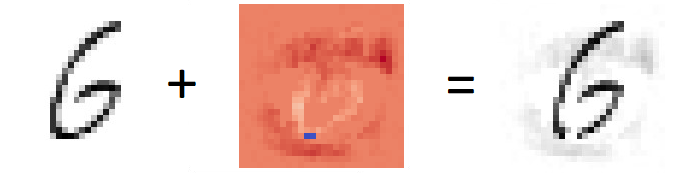
\includegraphics[width=10cm]{../images/six.png}
 \end{center}
 \begin{center}
	\pic{six}
	Початкове зображення класифікується нейронною мережею як ``шість''. Після додавання до нього певного шуму НМ класифікує його як ``п'ять''.
 \end{center}

 \subsection{Швидкий градієнтний спуск}

 Метод швидкого градієнтного спуску є одним з найпростіших методів генерації ошукуючих прикладів. Його застосовують для атак на різні системи машинного навчання, зокрема й на нейронні мережі \cite{explaining-a-e}.

 Основною метою методу є максимізація функції витрат $J$, розглядаючи її як $J(x, y_{true})$, зафіксувавши ваги нейронної мережі. В такому випадку потрібно знайти $x^{adv}$ таке, що виконується нерівність: 

 $$
 J\left(x^{adv}, y_{true}\right)>J\left(x, y_{true}\right)
 \eqno \n \label{convergency}
 $$
 Тоді, згідно з \cite{quarteroni}, ми зможемо знайти розв'язок поставленої задачі. Пошук ошукуючих зразків здійснюємо за формулою:
 $$
 x^{adv} = x + \epsilon {sign}\left(\nabla_x J\left(x, y_{true}\right)\right)
 \eqno \n \label{FGSM}
 $$
 де $\epsilon$ - додатний параметр, який називатимемо \textit{розміром кроку}. Напрямок ${sign}\left(\nabla_x J\left(x, y_{true}\right)\right)$ є \textit{напрямком зростання} для функції $J$.

 Варто зауважити, що метод не гарантує знаходження ошукуючого зразка, бо нерівність (\ref{convergency}) свідчить лише про збільшення функції правдоподібності. Тому в загальному випадку доцільно використовувати ітераційну форму методу. Також можна застосовувати інші методи, такі як \cite{C-and-W}, для того, щоб зменшити розмір шуму $\tau$.


 \subsection{Оптимізація нульового порядку}
 Більшість реальних систем, які використовують нейронні мережі, не розголошують своїх конфігурацій (як от структура мережі і її ваги), тому атаки, на кшталт швидкого градієнтного спуску не так просто застосувати на практиці. В деяких сценаріях зловмисники мають можливість використовувати модель для отримання передбачень на основі власних зразків (як от, наприклад, при використанні  програмних інтерфейсів від Google AI чи Amazon). Запити до мережі  дозволено повторювати необмежену кількість разів і на основі результатів покращувати ошукуючі зразки.

 Тоді є можливість обчислити градієнт наближено, для чого достатньо лише результату класифікації $f(x)$ та відповідного вхідного параметра $x$, як показано в \cite{zoo}. Якщо обчислимо часткові похідні наближено, за формулою

 $$
 \frac{\partial J(\mathbf{x})}{\partial \mathbf{x}_{i}} \approx
 \lim_{h \to 0} \frac{J\left(\mathbf{x}+h e_{i}\right)-J\left(\mathbf{x}-h e_{i}\right)}{2h},
 \eqno \n \label{df-zoo}
 $$
 де $e_i$ - вектор, в якому $i$-тий елемент дорівнює одиниці, а всі решта -- нулю, то зможемо застосувати для атаки на чорну скриньку алгоритми, що використовують похідні для розв'язання задачі оптимізації, такі як швидкий градієнтний спуск.

 При використанні наближених значень похідних в методі швидкого градієнта (\ref{FGSM}) вдається досягти результативності, близької до тої, яку отримуємо під час атак на білу скриньку. Це зумовлено тим, що для ефективної роботи методів достатньо лише знаку градієнту. Те, що значення обчислені з певною похибкою, значним чином не впливає на результат. Недоліком такого сценарію є необхідність виконувати класифікацію значну кількість разів, що займає багато часу та ресурсів і може бути легко виявлено.

 \subsection{Метод Карліні і Вагнера [TODO, optional]}
 \subsection{Перенесення ошукуючих зразків [TODO, optional]}
 
 \newpage
 \thispagestyle{empty}
 \section{Принципи захисту від ошукуючих атак}
 
 Як бачимо з попереднього розділу, для атак, які базуються на створенні ошукуючих зразків, характерним є використання градієнтів, обчислених для оцінки чутливості мережі до зміни вхідних даних. Такі градієнти також називають ошукуючими \cite{defencive-distillation}. Очевидно, що при великих значеннях ошукуючих градієнтів зловмиснику значно простіше знайти відповідний ошукуючий зразок для деякого вхідного зображення, бо невеликі збурення вхідного зразка призведуть до значної зміни результату передбачення.
 
 Таким чином, щоб збільшити стійкість мережі до ошукуючих атак, необхідно зменшити таку різку залежність від вхідних даних, а отже і амплітуду коливань ошукуючих градієнтів. Це означає що нам потрібно ``згладити'' модель, отриману під час стандартного процесу навчання, щоб допомогти їй краще узагальнювати зразки, які не є частиною тренувального набору.
 
 Варто звернути увагу на те, що ошукуючі зразки не обов'язково мають бути створені штучно на основі дослідження мережі-цілі, спеціально для того щоб отримати бажаний результат класифікації. У цьому розділі ми побачимо, що в ``природі'' таких прикладів також вдосталь, причому деякі неправильно натреновані нейронні мережі є до них особливо вразливими. 
 
 В попередніх розділах ми визначили надійність глибоких нейронних мереж як їх стійкість до обмежених збурень вхідних даних. Іншими словами, надійна модель повинна показувати високу точність не лише всередині навчального набору даних, а й за його межами, тобто моделювати функцію, яка ``інтуїтивно'' розподіляє віхідні дані між запропонованими категоріями в околі даного зразка. Цей окіл може бути визначений нормою у відповідному просторі.

 [TODO]
 \cite{analysis-of-robustness}
 Надійність використання норми при визначенні стійкості до атак 


 
 \begin{comment}
 [TODO]
 
 Отже, ошукуючі зразки не обов'язково витягуються з вхідного розподілу який ми намагаємось змоделювати під час навчання, використовуючи архітектуру DNN.
 
 \end{comment}
 
 
 
 \subsection{Боротьба з штучно створеним шумом ? природа ошукуючих зразків}
 \begin{center}
 	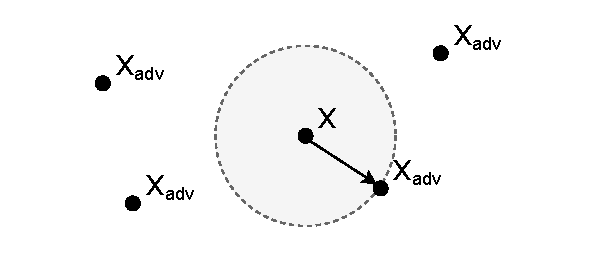
\includegraphics[width=12cm]{../images/2Dball.pdf}
 \end{center}
 \begin{center}
 	\pic{domain} 2D ілюстрація.
 \end{center}
 Не просто  знайти ефективний підхід до боротьби з ошукуючими збуреннями, при цьому не завдавши шкоди точність моделі.
 
 Adversarial training
 
 Example detection
 
 Generalization (зменшення розмірності)
 
 
 Додавання випадкового шуму
 
  
 \subsection{Надмірне тренування як причина вразливості}
 
 Працюючи ...
 На думку спадає ще один феномен у машинному навчанні, який має схожу причину -- \textit{перетренування (overfitting)}.
 
 І справді, бачимо залежність між стійкістю моделі та надмірним тренуванням. Перетреновані моделі надзвичайно вразливі до штучно створених ошукуючих зразків. Більше того, нівіть класифікація зразків з тестувального набору є для них складною задачею.
 
 Така поведінка зумовлена тим, що границя рішень .....
 
 
 
 \newpage
 \thispagestyle{empty}
 \section{Захисна дистиляція та її модифікації}
  В цьому розділі ми розглянемо підхід до оптимізації нейронної мережі або групи нейронних мереж, метою якого є зменшення обчислювальних затрат та ресурсів під час функціонування моделі. Це підхід був розроблений інженерами компанії Google Хілтоном на ін. і описаний в \cite{distillation}. Не зважаючи на те, що першочерговою метою дистиляції є зменшення розміру нейронної мережі щоб зробити можливим розгортання на пристроях з обмеженими ресурсами, згідно з \cite{defencive-distillation} її побічні ефекти можуть зробити мережу стійкішою до ошукуючих зразків.
 
 \subsection{Дистиляція нейронних мереж}
 
 Основна ідея методу дистиляції полягає у перенесенні знань з мережі прообразу за допомогою векторів імовірності приналежності зразка до деякого класу, отриманих використовуючи вже існуючу нейронну мережу. На основі цих даних тренується нова нейронна мережа з меншою розмірністю, при чому без значних втрат точності. Ця ідея базується на тому, що знання, здобуті моделлю під час тренування можна отримати не лише безпосередньо з ваг НМ, вони також ``закодовані'' в її передбаченнях.
 
 Як ми уже згадували раніше, кожен результат передбачення містить у собі деяку інформацію про модель. Таким чином вектори імовірності $\hat{y}$, отримані з одної моделі містять у собі достатньо інформації, щоб з їх допомогою можна було відтворити модель. Дистиляція ``витягує'' знання з цих векторів і переносить їх на модель з менш комплексною архітектурою.
 
 Використовуючи уже натреновану та готову до використання модель, кожному зразку тренувальних даних ставиться у відповідність вектор ймовірностей приналежності зразка до кожного з класів, які належать до предметної області моделі. Перевага використання таких прогнозів полягає у тому, що тепер кожна мітка містить не просто жорсткі оцінки, а інформацію про приналежність зразка до кожного з класів.
 
 %----------------------------------------------------------------------------------------------------------
 
 Процедура тренування прообразу не має строгих обмежені і нічим не відрізняється від звичних підходів. Наприклад, можна застосувати градієнтний спуск на даних з тренувального набору. Тепер можемо ввести поняття передавального набору.
 
 \begin{defn}
 	[TODO] Означення передавального набору.
 \end{defn}
 
 
 В найпростішій формі дистиляції знання переносяться до дистильованої моделі через тренування на вище згаданому передавальному наборі даних, використовуючи м'які мітки отримані при високих температурах вихідного шару моделі-оригіналу. Така ж температура використовується під час тренування дистильованої моделі, але після завершення процесу її повертають до стандартного значення, рівного одиниці.
 
 [TODO] Якісь припущення?
 
 Проблема цього підходу криється в тому, що точність моделі-прообраза завжди є менша за 100\%. Це означає, що передавальний набір буде містити деякі зразки з неправильними мітками і тренування на ньому нової моделі призведе до втрат точності на тестувальному наборі. Якщо відомі точні класи об'єктів, приклади з неправильними мітками варто виключити з передавального набору або замінити їх на правильні жорсткі мітки. Таким чином процес дистиляції може бути значно покращеним і точність моделі-образу залишиться на високому рівні.
 
 Ще один підхід до розв'язання проблем з передавальним набором наводять автори в \cite{distillation}. Під час тренування вони пропонують використовувати середнє арифметичне двох різних функцій оцінки. Перша з них -- функція крос ентропії [TODO] ref, обчислена з використанням такої ж високої температури $T$ в вихідному шарі НМ, яка використовується під час генерації м'яких міток. Друга функція оцінки -- функція крос ентропії з правильними жорсткими мітками при температурі $T=1$.
 
 [TODO] формула
 
 Оскільки величини градієнтів масштабуються з коефіцієнтом $\frac{1}{T^2}$, то варто домножити їх на $T^2$ при використанні як м'яких, так і жорстких міток. Це гарантує, що відносні частки вкладу м'якої та жорсткої міток залишатимуться приблизно незмінними, якщо температура буде змінюватися під час експериментів.
 
 [TODO] формула
 
 \subsection{Процес тренування та основні параметри} 
 
 \begin{center}
 	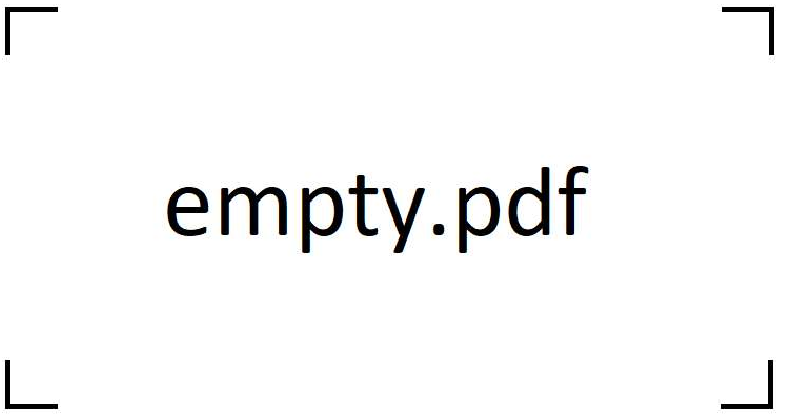
\includegraphics[width=10cm]{../images/empty.pdf}
 \end{center}
 \begin{center}
 	\pic{distilation} Схема тренування/ схема НМ.
 \end{center}
 
 Процес дистиляції розпочинається з підготовки мережі-прообразу, вихідний шар якої побудований на основі функції -- Softmax з врахуванням температури випаровування $T$.
 
 [TODO] ref Формула
  
 \begin{equation}
 \label{softmax-t}
 \hat{Y}(x)=\left(\frac{e^{z_{i}(x) / T}}{\sum\limits_{i=0}^{C-1} e^{z_{i}(X) / T}}\right)_{i \in 0 \dots C-1}
 \end{equation}

 У межах Softmax шару кожен нейрон відповідає класу за індексом $i \in 0 \dots С-1$ (де С - кількість класів) і обчислює відповідний компонент за формулою \ref{softmax-t}, де $Z(x) = z_0(X), \dots , z_{С-1}$ -- C логітів [TODO](перекласти/ перефразувати/ послатись на розділ про НМ), що відповідають виходу прихованого шару для кожного з С класів у наборі даних.
 
 Параметр $T$ також називають температурою дистиляції. Він $T$ впливає на те, наскільки елементи вектору ймовірностей $\hat{y}$ будуть відрізнятись один від одного. 
 
 [TODO] Температура відіграє центральну роль у основних явищах дистиляції, що ми покажемо пізніше у цьому розділі.
 
 Так при малих $T$ різниця між ймовірностями буде значною, тобто один із елементів вектора буде сильно виділятись з-поміж інших. В свою чергу, висока температура змушує НМ створювати ймовірнісні вектори з відносно великими значеннями для кожного класу.
 
 \begin{center}
 	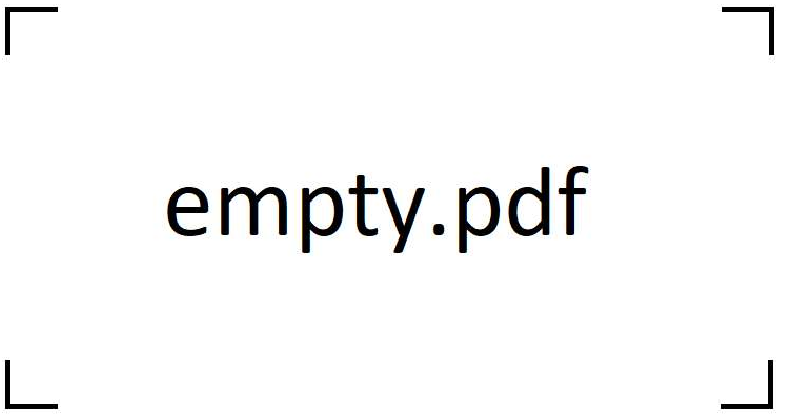
\includegraphics[width=10cm]{../images/empty.pdf}
 \end{center}
 \begin{center}
 	\pic{distilation} Залежність ймовірностей для конкретного класу від температури дистиляції [TODO] bar plots.
 \end{center}
 
 Дійсно, при високій температурі, логіти у векторі Z(x) стають незначними
 у порівнянні з температурою $Т$. Тому всі компоненти
 вектор імовірності $\hat{Y}(X)$, виражені у рівнянні (\ref{softmax-t}) прямують до 
 $1/C$ при $T \to \inf$ . Чим вища температура,
 тим більш неоднозначним буде розподіл ймовірностей (тобто всі
 ймовірності виходу $\hat{Y}(X)$ близькі до $1/C$), тоді як
 при малій температурі розподіл буде більш дискретним (тобто одна з ймовірностей у
 виході $\hat{Y}(X)$ буде близькою до 1, а решта -- близькі до 0).
 
 
 На основі векторів ймовірності, створених першою НМ, формується передавальний набір
 
 
 \begin{comment}
 Тоді вектори ймовірності, створені першим DNN, є
 використовується для позначення набору даних. Ці нові мітки називаються м'якими
 етикетки на відміну від ярликів жорсткого класу. Друга мережа з
 тоді менше одиниць навчається за допомогою цього нещодавно позначеного набору даних.
 Як варіант, другу мережу також можна навчити, використовуючи
 поєднання міток жорсткого класу та вектора ймовірностей
 етикетки. Це дозволяє мережі користуватися обома ярликами
 сходитися до оптимального рішення. Знову другий
 мережа тренується при високій температурі softmax, ідентичній
 той, що використовується в першій мережі. Однак ця друга модель
 меншого розміру, досягає порівнянної точності, ніж оригінал
 модель, але є менш обчислювально обчислювальною. Температура
 повертається до 1 під час тестування, щоб отримати більше дискретного
 вектори ймовірності під час класифікації.
 \end{comment}
 
 \subsection{Оцінка захисту}
 
 Фільтрований передавальний набір vs не філтрований
 
 \newpage
 \thispagestyle{empty}
 \section{Методи з гарантованою стійкістю}
 Основна проблема багатьох методів захисту, зокрема і розглянутої раніше захисної дистиляції полягає в тому, що їх ефективність важко, або навіть неможливо довести теоретично. Через це часто виникають випадки, коли захист моделі є ефективним лише для конкретних задач і проти конкретних методів атаки,
 як, наприклад, в [TODO] cite distilation is not robust. Тому цінними є методи, при використанні яких можна гарантувати певний рівень стійкості. Такі методи захисту також називають \textit{сертифікованими}. Один з таких методів ми і роглянемо в даному розділі. Він називається \textit{PixelDP} і був запропонований  запропонований Матіасом Лекуєром та ін. в \cite{pixeldp}. Він базується на принципі \textit{диференційованої конфіденційності (differential privacy)}, в основі якого лежить рандомізація обчислень на великих масивах даних \cite{differential-privacy}.
 
 [TODO]
 \subsection{Захист PixelDP}
 
 \begin{center}
 	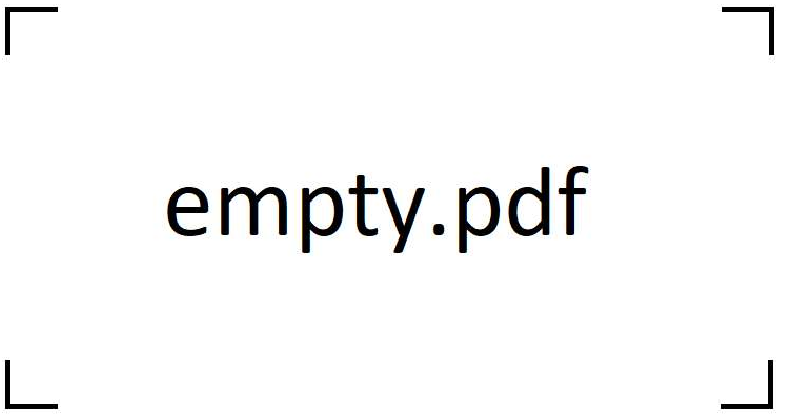
\includegraphics[width=10cm]{../images/empty.pdf}
 \end{center}
 \begin{center}
 	\pic{distilation} Схема тренування/ схема НМ.
 \end{center}
 
 
 \subsection{Оцінка захисту}
 
 \newpage
 \thispagestyle{empty}
 \section{Комбінація методів та побудова архітектури, стійкої до атак}
 
 \newpage
 \thispagestyle{empty}
 \section{Експерименти?}
 
 
 
 \newpage
 \thispagestyle{empty}
 \addcontentsline{toc}{section}{Висновок}
 \section*{Висновок}
 
 \newpage
 \thispagestyle{empty}
 \addcontentsline{toc}{section}{Додатки}
 \section*{Додатки}
 
 \textit{Додаток 1.} Деякі приклади ошукуючих зразків
 
 \textit{Додаток 2.} Таблиці про нм?
 
 \textit{Додаток 3.} Нм для розпізнавання цифр [TODO](prev work)
 
 \textit{Додаток}

 \newpage
 \thispagestyle{empty}
 \addcontentsline{toc}{section}{Література}
 \begin{thebibliography}{99}
	
	\bibitem[1]{first-work}
	\textit{Christian Szegedy, Wojciech Zaremba, Ilya Sutskever, Joan Bruna, Dumitru Erhan, Ian Goodfellow, Rob Fergus} /
	Intriguing properties of neural networks /
	arXiv preprint arXiv:1312.6199 (2014)
	
	\bibitem[2]{defencive-distillation}
	\textit{Nicolas Papernot, Patrick McDaniel, Xi Wu Somesh Jha,Ananthram Swami} /
	Distillation as a Defense to Adversarial Perturbations against Deep Neural Networks /
	arXiv preprint arXiv:1511.04508 (2016)
	
	\bibitem[3]{distillation}
	\textit{Geoffrey Hinton, Oriol Vinyals, Jeff Dean} /
	Distilling the Knowledge in a Neural Network /
	arXiv preprint arXiv:1503.02531 (2015)
	
	\bibitem[4]{pixeldp}
	\textit{Mathias Lecuyer, Vaggelis Atlidakis, Roxana Geambasu, Daniel Hsu, Suman Jana} /
	Certified Robustness to Adversarial Examples with Differential Privacy/
	arXiv preprint arXiv:1802.03471 (2019)
	
	\bibitem[5]{analysis-of-robustness}
	\textit{Alhussein Fawzi, Omar Fawzi, Pascal Frossard} /
	Analysis of classifiers' robustness to adversarial perturbations /
	arXiv preprint arXiv:1502.02590 (2016)
	
	\bibitem[6]{ensemble}
	\textit{Thamas G. Dietterich} /
	Ensemble Methods in Machine Learning /
	Springer (2000)
	
	\bibitem[7]{differential-privacy}
	\textit{Cynthia Dwork} /
	Differential Privacy /
	Automata, Languages and Programming. ICALP (2006)
	
	\bibitem[8]{explaining-a-e}
	\textit{Ian Goodfellow, Jonathon Shlens, Christian Szegedy} /
	Explaining and Harnessing Adversarial Examples /
	arXiv preprint arXiv:1412.6572 (2014)
	
	\bibitem[9]{quarteroni}
	\textit{Alfio Quarteroni, Riccardo Sacco, Fausto Saleri} /
	Numerical Mathematics / --
	Springer, 2000. --300 p.
	
	\bibitem[10]{black-box-2}
	\textit{Nicolas Papernot, Patrick McDaniel, Ian Goodfellow} /
	Transferability in machine learning: from phenomena to black-box attacks using adversarial samples /
	arXiv preprint arXiv:1605.07277 (2016)
	
	\bibitem[11]{zoo}
	\textit{Pin-Yu Chen, Huan Zhang, Yash Sharma, Jinfeng Yi, Cho-Jui Hsieh} /
	ZOO: Zeroth Order Optimization Based Black-box Attacks to Deep Neural Networks without Training Substitute Models /
	arXiv preprint arXiv:1708.03999 (2017)
	
	\bibitem[12]{C-and-W}
	\textit{Nicholas Carlini, David Wagner} /
	Towards Evaluating the Robustness of Neural Networks /
	arXiv preprint arXiv:1608.04644 (2017)
	
	\bibitem[13]{my-work}
	\textit{Богдан Бугрій, Юрій Музичук} /
	Атаки на глибокі нейронні мережі /
	(2020)
	
	
 \end{thebibliography}

 \end{document}

